\documentclass[a4paper,12pt]{article}

\usepackage[utf8]{inputenc}
\usepackage[english,russian]{babel}
\usepackage{indentfirst}
\usepackage{misccorr}
\usepackage{float}
\usepackage{graphicx}
\usepackage{gensymb}
\DeclareGraphicsExtensions{.pdf,.png,.jpg}
\graphicspath{{/}}
\usepackage{amsmath}

\begin{document}

\title{Проверка теоретической зависимости температуры длинного тела от расстояния до источника тепла}
\author{Ахундзянов Амир Андреевич, Цветков Пётр Алексеевич}
\date{\today}
\maketitle

\section{Задачи и цели}

Цель данного эксперимента - проверить теоретически полученную экспоненциальную зависимость установившейся температуры стержня от расстояния до нагревателя при условии теплообмена с окружающей средой. Выяснить по набору экспериментальных данных коэффициенты зависимости.


\section{Теоретическое обоснование}

На уроке экспериментальной физики была выведена теоретическая зависимость: 
{\Large $$T(x) = (T_1 - T_0) \cdot e ^ {- x \cdot \sqrt{\frac{2}{\varkappa \rho r}}} + T_0$$}
Где: 
\begin{itemize}
\item $T_0$ - температура окружающей среды (в нашем случае воздуха в комнате)
\item $T_1$ - температура нагревателя (в нашем случае плитки)
\item $\varkappa$ - коэффициент теплопроводности материала стержня
\item $\rho$ - коэффициент, характеризующий передачу тепла от стержня к внешней среде (воздуху)
\end{itemize}
Обозначим $K = \varkappa \cdot \rho$ - по формуле имеет размерность длины. Будем искать из эксперимента $T_0, T_1, K$.

\section{Методика и оборудование}
Оборудование - горячая плитка, металлический стержень, мультиметр с термопарой, линейка, карандаш, штатив. \\\\

Метод проведения эксперимента - разметить поршень по длине с помощью линейки. Положить край стержня на плитку, второй края зафиксировать на штативе. Дождаться установления теплового равновесия. Замерить температуру стержня термопарой на разных отметках. Результаты записать в таблицу, с помощью программы Excel подобрать оптимальные коэффициенты теоретической зависимости. Результаты визуализировать на графике.

\section{Результаты измерений и обработка данных}

После обработки в программе Excel были получены коэффициенты, при которых теоретическая функция наиболее точно описывает результаты эксперимента:
\begin{itemize}
\item $T_0 = 28.2$ $^oC$
\item $T_1 = 146.5$ $^oC$
\item $K = 2,34$ м
\end{itemize}

Полученные результаты изображены на графике на рисунке \ref{fig:viz}.

\begin{figure}[H]
\centering
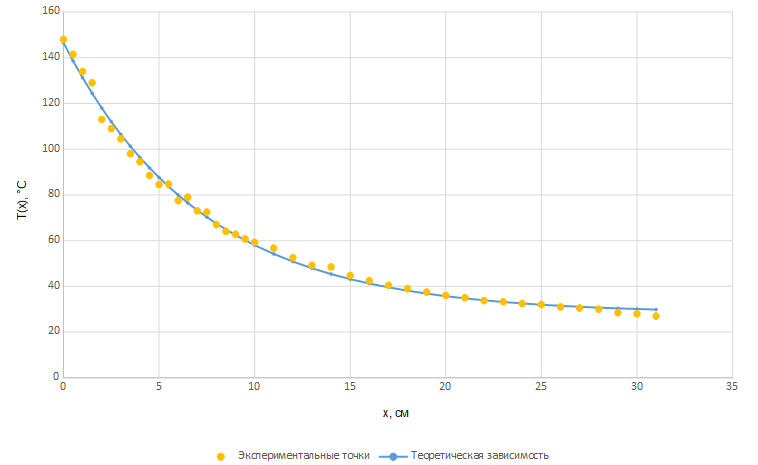
\includegraphics[width=1.1\textwidth]{chart}
\caption{Визуализация обработанных данных}
\label{fig:viz}
\end{figure}

\section{Вывод}


Проведя эксперимент и проанализировав полученные результаты, мы пришли к выводу, что теоретическая модель, полученная на уроке хорошо описывает физические явления, наблюдаемые при нагревании металлического стержня в реальном мир.


\end{document}